\documentclass[11pt,a4paper]{ctexart}

\usepackage[margin=2.6cm]{geometry}
\usepackage{amsmath,amssymb,amsthm}
\usepackage{graphicx}
\usepackage{booktabs}
\usepackage{hyperref}
\usepackage{xcolor}
\usepackage{listings}
\usepackage{caption}

\graphicspath{{figures/}}
\hypersetup{colorlinks=true, linkcolor=blue!50!black, urlcolor=blue!60!black}
\lstset{
  basicstyle=\ttfamily\small,
  breaklines=true,
  frame=single,
  columns=fullflexible,
  backgroundcolor=\color{gray!7}
}

\newtheorem{definition}{定义}[section]
\newtheorem{theorem}{定理}[section]
\newtheorem{lemma}{引理}[section]
\newtheorem{proposition}{命题}[section]
\newtheorem{example}{例}[section]

\title{第 9 章 \quad Parameter estimation / 参数估计}
\author{基于 \textit{A Course in Time Series Analysis} 的中文讲义与 Python 实践}
\date{}

\begin{document}
\maketitle

\section*{本章学习目标}

本章按照原文 \textit{Parameter estimation} 的小节顺序整理，保留主要定义、定理、模型公式和练习方向，并将原文中的 R 实践思路改写为 Python 工程实践。

完成本章后，应能够：
\begin{itemize}
  \item 掌握 AR 模型的 Yule-Walker、条件最小二乘和高斯似然估计；
  \item 理解 Burg 算法与偏自相关递推；
  \item 描述 AR 估计量的抽样性质；
  \item 掌握 ARMA 的精确/近似高斯似然和 Kalman 滤波估计；
  \item 了解 Hannan-Rissanen 与 ARCH 准最大似然。
\end{itemize}

\section{自回归模型估计}

AR(p) 模型为
\[
  X_t=\phi_1X_{t-1}+\cdots+\phi_pX_{t-p}+\varepsilon_t.
\]
\subsection{Yule-Walker 估计}

理论方程为
\[
  \Gamma_p\phi=\gamma_p,
\]
其中 \(\Gamma_p=(c(i-j))_{i,j=1}^p\)，\(\gamma_p=(c(1),\ldots,c(p))'\)。用样本自协方差替代即可得
\[
  \hat\phi_{YW}=\hat\Gamma_p^{-1}\hat\gamma_p.
\]

\subsection{高斯似然}

若 \(X=(X_1,\ldots,X_n)'\sim N(0,\Sigma_\theta)\)，高斯负对数似然差一个常数为
\[
  \ell(\theta)=\log|\Sigma_\theta|+X'\Sigma_\theta^{-1}X.
\]
该形式精确但计算协方差矩阵和逆矩阵成本较高。

\section{条件高斯似然与最小二乘}

条件在初始 \(X_1,\ldots,X_p\) 上，AR(p) 的条件残差为
\[
  e_t(\phi)=X_t-\phi_1X_{t-1}-\cdots-\phi_pX_{t-p}.
\]
条件最小二乘估计为
\[
  \hat\phi_{CLS}
  =\arg\min_\phi\sum_{t=p+1}^n e_t(\phi)^2.
\]
它把 AR 估计转化为普通回归问题。

\subsection{Burg 算法}

Burg 算法通过同时最小化前向和后向预测误差估计反射系数，保证估计得到的 AR 模型稳定。其递推与 Levinson-Durbin 和 PACF 紧密相关。

\section{AR 估计量的抽样性质}

\begin{definition}[鞅差，原文 Definition 9.1.1]
若 \(E(Z_t\mid\mathcal F_{t-1})=0\)，则称 \(\{Z_t\}\) 为鞅差序列。
\end{definition}

在稳定 AR 模型和适当矩条件下，Yule-Walker、条件最小二乘和高斯似然估计量通常相合且渐近正态：
\[
  \sqrt n(\hat\phi-\phi_0)\Rightarrow N(0,V).
\]
证明核心是把估计方程展开为鞅差和可忽略项。

\section{ARMA 模型估计}

ARMA(p,q)
\[
  \phi(B)X_t=\theta(B)\varepsilon_t
\]
的似然需要根据参数递归计算创新。常见方法包括精确高斯最大似然、近似高斯似然和 Kalman 滤波。

\begin{theorem}[ARMA GMLE 抽样性质，原文 Theorem 9.2.1]
在因果、可逆、可识别和矩条件下，ARMA 高斯最大似然估计量相合并渐近正态。
\end{theorem}

\subsection{Hannan-Rissanen 方法}

该方法先用高阶 AR 近似 ARMA 的 \(AR(\infty)\) 表示，估计创新，再用回归估计 ARMA 参数，是一种计算上较快的初值或估计方案。

\section{ARCH 准最大似然}

ARCH/GARCH 中即使创新非高斯，也常使用高斯准似然。只要条件均值和条件方差设定正确，参数仍可具有良好渐近性质。

\section{原文定理、例题与算法补充}

\subsection{Yule-Walker 技术引理}
\begin{lemma}[原文 Lemma 9.1.1]
对零均值随机向量 \(Z\)，二次型和协方差矩阵的性质可用于控制 Yule-Walker 估计误差。这一引理服务于 AR 参数估计量的抽样性质。
\end{lemma}

\subsection{AR(1) 高斯似然例题}
\begin{example}[原文 Example 9.1.1]
在 AR(1) 情形，协方差矩阵和条件分布都可显式写出，因此能直接看出精确高斯似然与条件似然之间的差别。
\end{example}

\subsection{Yule-Walker 与最小二乘玩具例子}
\begin{example}[原文 Example 9.1.2]
原文用一个小例子比较 Yule-Walker 与最小二乘。二者都估计 AR 参数，但一个从样本协方差方程出发，另一个从预测残差平方和出发。
\end{example}

\subsection{AR 估计量渐近理论}
\begin{theorem}[原文 Theorem 9.1.1]
在鞅差和矩条件下，AR 估计方程的主项满足中心极限定理，从而得到参数估计量的渐近正态性。
\end{theorem}

\subsection{ARMA 最大似然与 Hannan-Rissanen}
\begin{theorem}[原文 Theorem 9.2.1]
若 ARMA 模型因果、可逆、可识别且满足矩条件，高斯最大似然估计量相合并渐近正态。
\end{theorem}

Exercise 9.1 要求用普通最小二乘估计 AR 参数并与软件输出比较；Exercise 9.2 研究随机自回归模型的参数估计。Burg 算法、Kalman 似然和 Hannan-Rissanen 方法共同构成 ARMA 估计的实用工具箱。

\section{Python 工程实践}

在本章目录下运行：
\begin{lstlisting}[language=bash]
python scripts/ch09_generate_figures.py
\end{lstlisting}

脚本会把图像写入本章 \texttt{figures/} 目录。当前图像用于配合本章核心概念的仿真说明；若后续补齐原始数据文件，可把模拟数据替换为原文真实数据案例。

\begin{figure}[htbp]
  \centering
  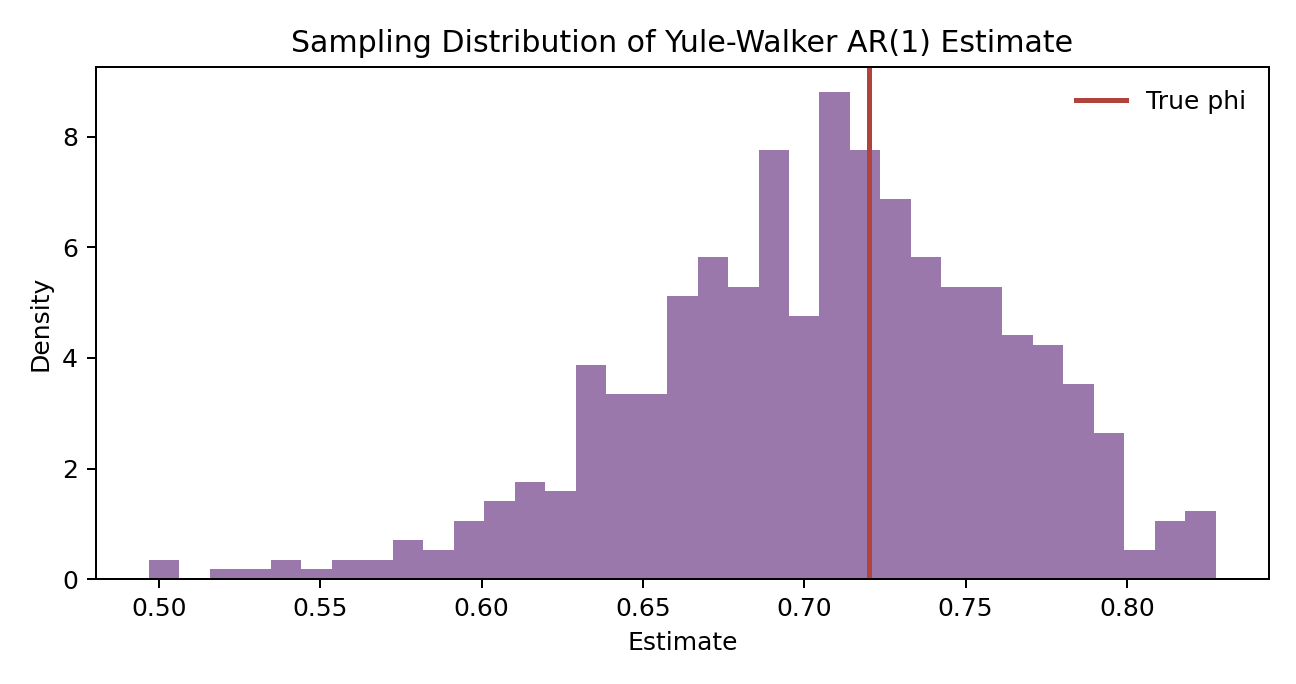
\includegraphics[width=0.86\textwidth]{ch09_fig01_yule_walker_sampling.png}
  \caption{Yule-Walker AR(1) 估计量的抽样分布：样本量有限时估计量围绕真值波动。}
\end{figure}

\begin{figure}[htbp]
  \centering
  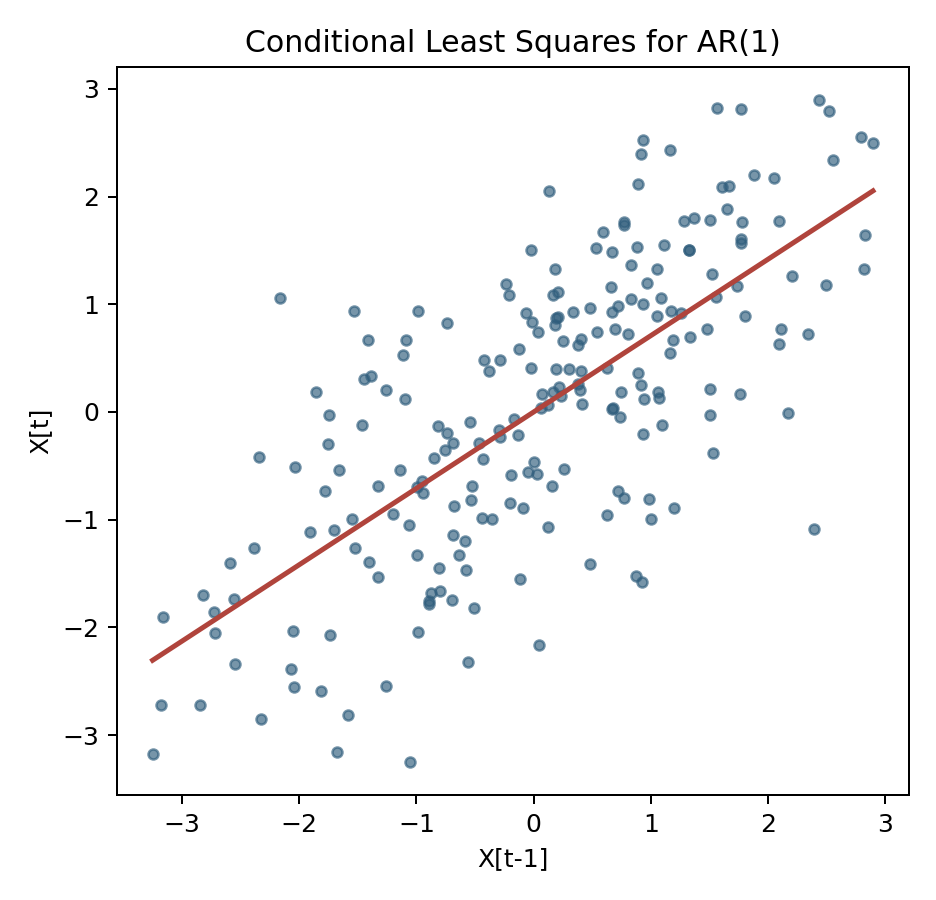
\includegraphics[width=0.86\textwidth]{ch09_fig02_cls_ar1.png}
  \caption{AR(1) 条件最小二乘：把 \(X_t\) 对 \(X_{t-1}\) 做回归得到参数估计。}
\end{figure}

\section{练习提要}

原文练习主要围绕下列方向展开：
\begin{itemize}
  \item 用 OLS、Yule-Walker 和 MLE 估计同一 AR 模型并比较；
  \item 推导 AR(1) 高斯似然的简单形式；
  \item 实现 Burg 算法或调用库函数比较结果；
  \item 估计随机系数 AR 或 ARCH 模型。
\end{itemize}

\section*{本章小结}

第 9 章集中讨论模型参数如何从数据中估计。AR 模型可由协方差方程、回归或似然估计；ARMA 估计更依赖创新递推和数值优化；渐近理论则解释估计误差如何随样本量缩小。

\end{document}
